\documentclass{beamer}
\newcommand{\vecnabla}{\vec{\nabla}}
% code
\newcommand{\code}[1]{
	\texttt{#1}
}
\usetheme{metropolis}  
\setbeamertemplate{bibliography item}{\insertbiblabel}
%\beamerdefaultoverlayspecification{<+->}
\usepackage{outlines}



\title{An FPGA-based Intel 8080 Mockup Soft Microprocessor}
\date{\today}
\author{Leonardo Cattarin}
\institute{University of Trento}

\begin{document}
  \maketitle
  \setbeamercovered{transparent}


  \begin{frame}{Modules scheme}
    \begin{figure}[hbtp]
      \centering
      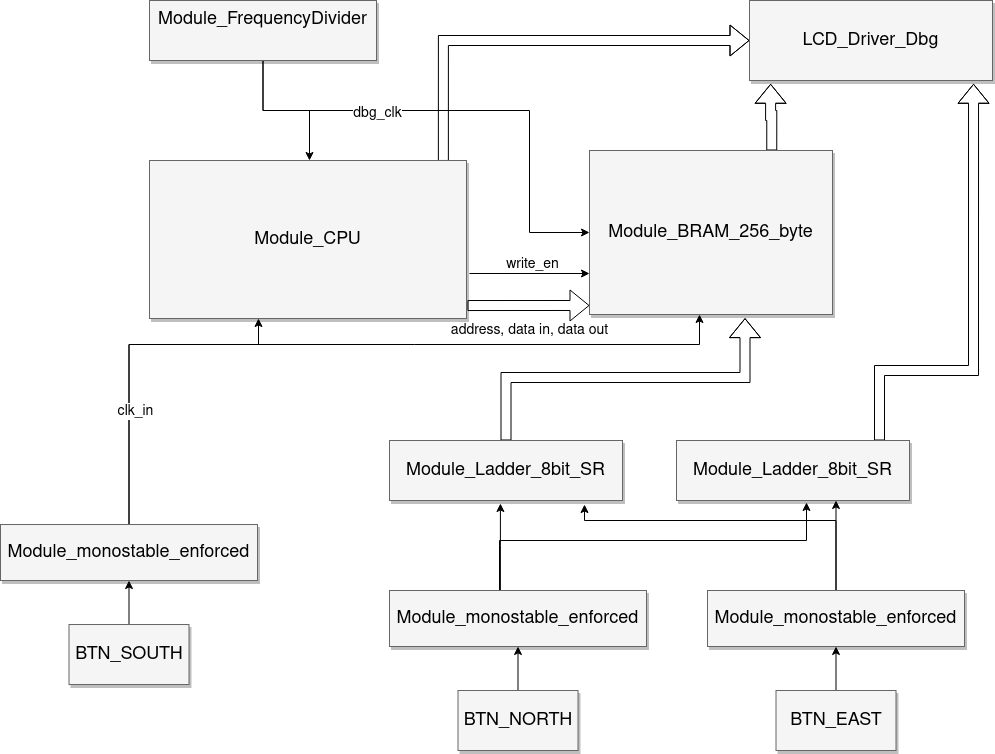
\includegraphics[width=0.9\textwidth]{img/System.png}
      \caption{Modules scheme of the computing system}
      \label{fig:system}
  \end{figure}
  \end{frame}

  \begin{frame}{CPU: Instruction Fetch-execute cycle}
    \begin{figure}[hbtp]
      \centering
      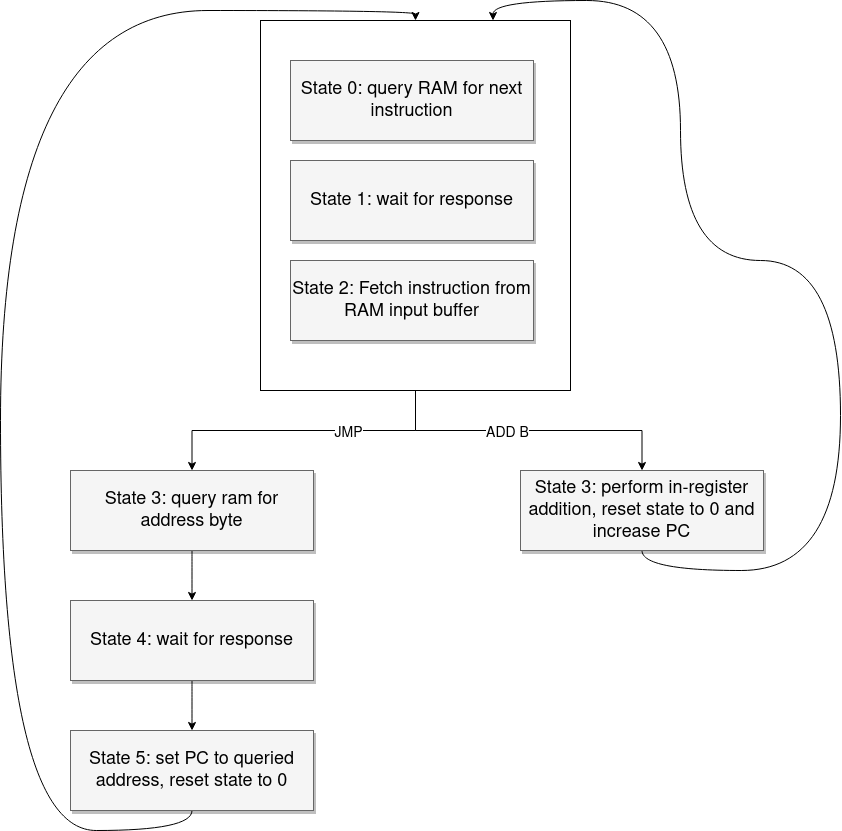
\includegraphics[width=0.7\textwidth]{img/States.png}
      \caption{Fetch-execute cycle corresponding to JMP and ADD instructions}
      \label{fig:diagram}
  \end{figure}
  \end{frame}

  \begin{frame}{CPU: Registers }
    \begin{itemize}
      \item \code{PC}: (8-bit) Program Counter, memory address to the next instruction.
      \item \code{IR}: (8-bit) Instruction Register, opcode of current instruction 
      \item \code{A,B,C}: (8-bit) General purpose registers 
      \item \code{W,Z}: (8-bit) Temporary registers 
      \item \code{H,L}: (8-bit) Registers used to store memory addresses
      \item \code{data\_addr,data\_out,write\_en}: Registers connected to output wirebuses.
      \item \code{flg\_carry},\code{flg\_sign},\code{flg\_zero},\code{flg\_parity},\code{flg\_auxiliary}: flag registers
  \end{itemize}

  \end{frame}

  \begin{frame}{CPU: instructions}
  \begin{itemize}
    \item \code{NOP}: do nothin 
    \item \code{JMP XX}: jump to address XX
    \item \code{JC XX}: jump if \code{flg\_auxiliary}=1
    \item \code{MVI B, XX}: copy immediately byte XX to B
    \item \code{MOV B,A}: \code{MOV B,C},\code{MOV C,B}, \code{MOV B,H}
    \code{MOV H,B}: \code{MOV B,L}, \code{MOV L,B}, \code{MOV M(H),B}, \code{MOV B,M(H)}, 
     copy operations
    \item \code{ADD B}: \code{ADD M[H]}, Add to content to A
    \item \code{CMP B}: compare A with B. If A=B, set zero flag to 1. Otherwise set it to zero, and set carry flag to zero if A>=B
    or 1 otherwise
    \item \code{CHC}: \code{CHZ}, \code{CHS}, \code{CHP}, copy content of flag registers auxiliary one.
    \item \code{HLT}: do noting and stop
\end{itemize}
\end{frame}



  \begin{frame}{RAM and LCD Display}
    \code{Module\_BRAM\_256\_byte} Module:
\begin{itemize}
  \item Based on Block RAM functionality of Spartan 3A
  \item Used as an array of 8-bit registers
  \item Used only 256 bytes = 8-bit addresses
  \end{itemize}
  

  \code{LCD\_Driver\_Dbg} module:
  \begin{itemize}
    \item Configures LCD display and issues a cycle of write commands
    \item Can show either RAM memory or CPU registers contens
    \item selectable via switch and pushbuttons
  \end{itemize}
  
\end{frame}




  \begin{frame}{Exampe: For loop}
    \begin{figure}[hbtp]
      \centering
      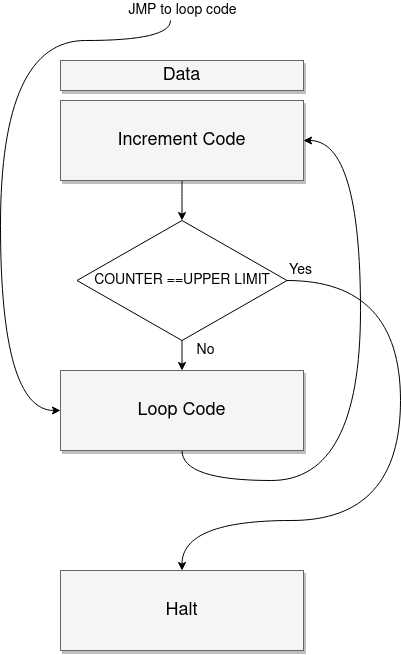
\includegraphics[width=0.4\textwidth]{img/Loop.png}
      \caption{Loop Example Scheme}
      \label{fig:system}
  \end{figure}
  \end{frame}



  \begin{frame}[fragile]{Exampe: For loop}
    \fontsize{6pt}{5.2}\selectfont
    \begin{columns}
      \begin{column}{0.5\textwidth}
      \begin{verbatim}
      //jump directly to loop instructions
      JMP PTR[LOOP]
      
      //initial counter value, upper limit 
      //and memory location to write numbers.
      COUNTER = 0 
      UPPER_LIMIT = 0A
      NUMBERS_ADDR = 35
      
      //code section for counter increment
      //and conditional jump
      #INCREMENT# 
      
      //load counter address in H
      MVI B,PTR[COUNTER] 
      MOV H,B 
      
      //put 01 in B, use it to increase counter by 1,
      // put result in B
      MVI B, 01 
      ADD B 
      MOV B,A 
      
      //write counter to its memory position
      MOV M[H],B  
      
      //load upper limit memory location in B
      // and then the limit itself
      MVI B,PTR[UPPER_LIMIT] 
      MOV H,B 
      MOV B,M[H] 

      //compare A (counter) with B(upper limit)
      //if A=B, zero flag is set to 1
      CMP B 
      \end{verbatim}
         \end{column}
      \begin{column}{0.7\textwidth}  %%<--- here
          \begin{verbatim}
            //check if zero flag is 1 (A=B) 
            //and jump to end program if true
            CHZ 
            JC PTR[AFTER_LOOP]
            
            #LOOP#
            //puts counter address in H
            MVI B,PTR[COUNTER]
            MOV H,B
            
            //puts counter in B, A and C
            MOV B, M[H]
            MOV A,B
            MOV C,B
            
            //load starting address for numbers writing
            MVI B,PTR[NUMBERS_ADDR]
            MOV H,B
            MOV B,M[H]
            
            //calculates address to write counter value, put in H
            ADD B
            MOV B,A
            MOV H,B
            
            //re-load counter value in B and A from C 
            //and write it to memory
            MOV B,C
            MOV A,B
            MOV M[H],B
            
            //jump to increment routine
            JMP [INCREMENT]
            
            #AFTER_LOOP# 
            HLT
            
            #NUMBERS_ADDR#
          \end{verbatim}
      \end{column}
      \end{columns}
  \end{frame}
  

\section{Bibliography}
\begin{frame}
  \cite{Assembly}
  \cite{Board}
  \cite{BRAM}
 \end{frame}
     

     \begin{frame}[allowframebreaks]
      \frametitle{References}
      \bibliographystyle{plain}
      \bibliography{bibliography.bib}
    \end{frame}

  
\end{document}